\documentclass{article}
\usepackage[T1]{fontenc}

\usepackage{graphicx}
\usepackage{listings}
\begin{document}

\title{FOSS Lab Report}
\author{Gokul K\\[2\baselineskip]
Roll Number: 21\\[2\baselineskip]}
\date{02 February 2020}

\maketitle

\setcounter{section}{10}
\section{Shell Programming VII}
\subsection{Aim}
Write a script that compares two directories dir1 and dir2(supplied as
arguments) and copies to dir1 from dir2 every file that is not present in
dir1.


\subsection{Source Code}
\begin{verbatim}
    #! /bin/bash

    # Gokul K
    # Roll No: 21
    # 25-01-2020

    # Write a script that compares two directories dir1 and dir2(supplied as
    # arguments) and copies to dir1 from dir2 every file that is not present in
    # dir1.

    if [[ $# -ne 2 ]]
    then
        echo "Insufficient number of arguments"
        exit
    fi

    if [[ !(-d $1) || !(-d $2) ]]
    then
        echo "Invalid arguments. Please enter directory names"
        exit
    fi

    diff $1 $2 | grep "$1" | awk '{for(i = 4; i <= NF; i++) printf "%s ",$i; printf "\n"}' |
    while read filename
    do
        cp "$1/$filename" $2
        echo "Copied $filename"
    done
\end{verbatim}

\subsection{Program Description}
diff command is used to find the differences in directories or files. Here
the two folders given as input is given as argument to a diff command and
the files found only in the first dir is copied to the second.

\subsection{Output}
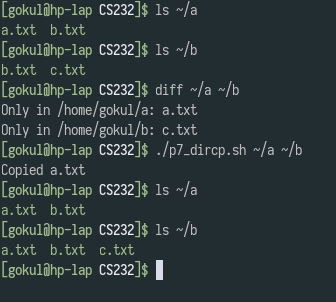
\includegraphics[width=0.9\textwidth]{img/p11.png}\newline

\subsection{Result}
The above program is run on Manjaro Linux shell. The unique files is directory 1
is copied to directory 2.
\end{document}